\section{Network-Wrapper}

Um in einer Flutter-App Requests sowie Responses über das \textit{HTTP}-Protokoll versenden und empfangen zu können
muss das von Dart bereitgestellte \textit{http}-Package zu den Dependencies im \lstinline{pubspec.yaml}-File hinzugefügt
werden.

\begin{code}
    \centering
    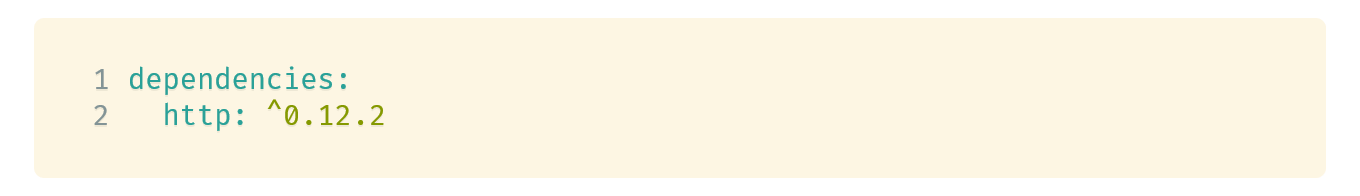
\includegraphics[width=1\textwidth]{images/Dart/util/network-wrapper/dependency.png}
    \caption{Hinzufügen des \textbf{http}-Packages zum \lstinline{pubspec.yaml}-File}
\end{code}

Mithilfe dieses Packages können nun \textit{GET}- und \textit{POST}-Requests an eine bestimmte URL, in unserem Fall
an die Sokka-API gesendet werden, wobei die erhaltene Antwort per \lstinline{jsonDecode()}-Funktion in ein lesbares
JSON-Format umgewandelt werden muss.

\begin{code}
    \centering
    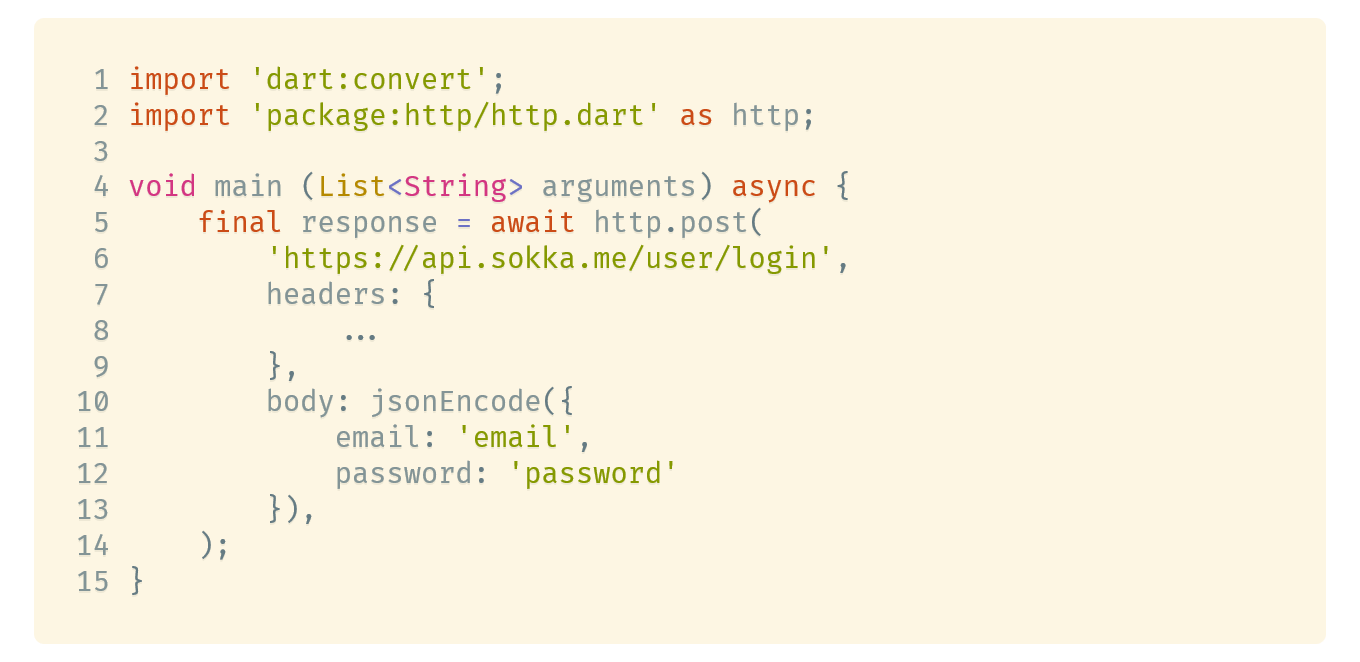
\includegraphics[width=1\textwidth]{images/Dart/util/network-wrapper/postRequest.png}
    \caption{Simples Beispiel für einen POST-Request}
\end{code}

\newpage

Um das Versenden und Verarbeiten solcher HTTP-Requests möglichst einfach zu gestalten bietet jene
Klasse zwei Wrapper-Funktionen für GET- und POST-Requests an.

Jene Funktionen erhalten die \textit{Ziel-URL} und entsprechendend \textit{Request-Headers} und \textit{-Body} in Form einer HashMap
als Argumente, welche direkt per \lstinline{jsonEncode()} umgewandelt werden.

Tritt bei einem durchgeführten Request ein Fehler auf - ein Statuscode der Antwort unter 200 bzw. über 400 oder ein
leeres JSON-Objekt - wirft die Funktion eine Exception mit entsprechendem HTTP-Code.

Erfolgt der Request fehlerlos so wird dessen Body per \lstinline{jsonDecode()} umgewandelt und retourniert.

\subsubsection{NetworkWrapper.GET}

\begin{code}
    \centering
    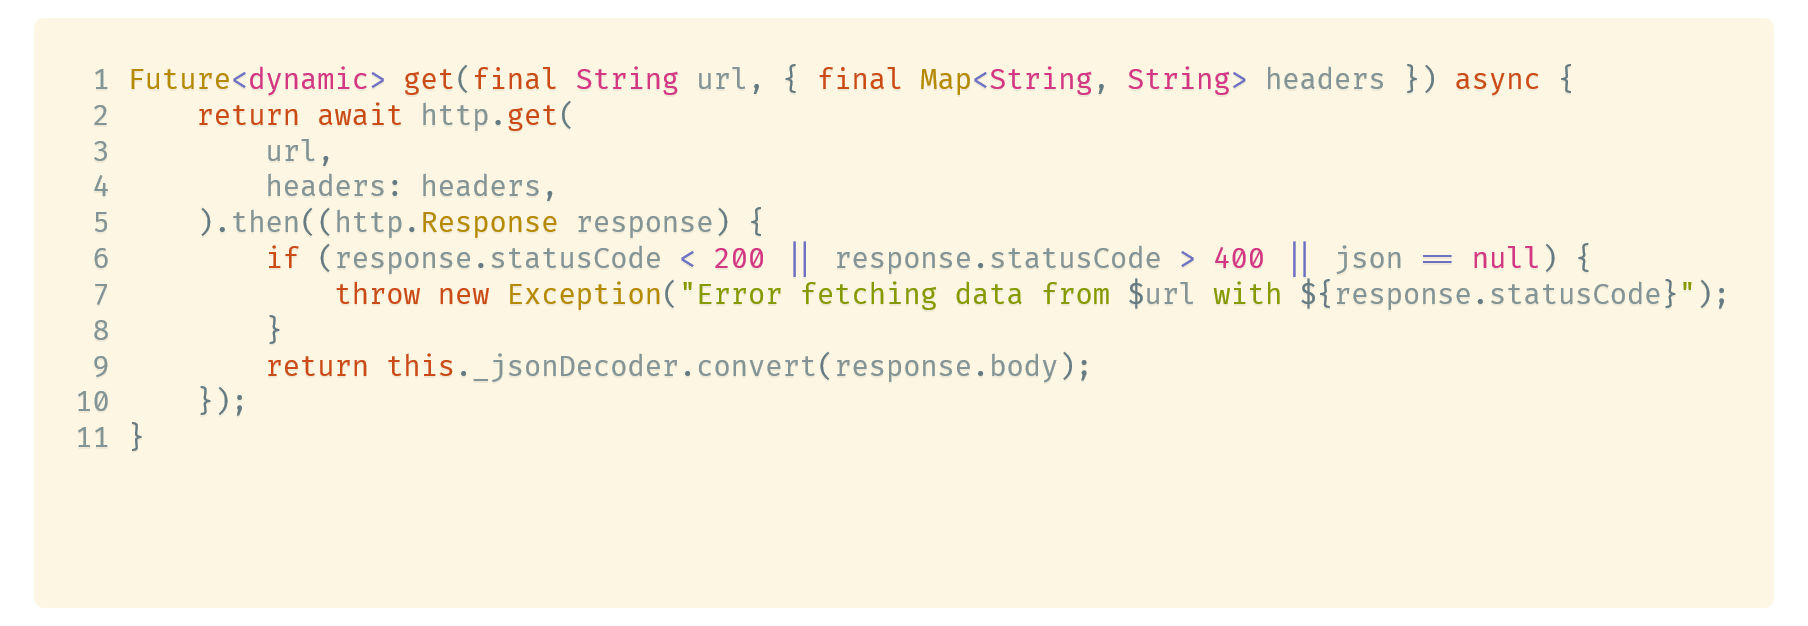
\includegraphics[width=1\textwidth]{images/Dart/util/network-wrapper/networkWrapperGET.png}
    \caption{GET-Request-Wrapper der NetworkWrapper-Klasse}
\end{code}

\subsubsection{NetworkWrapper.POST}

\begin{code}
    \centering
    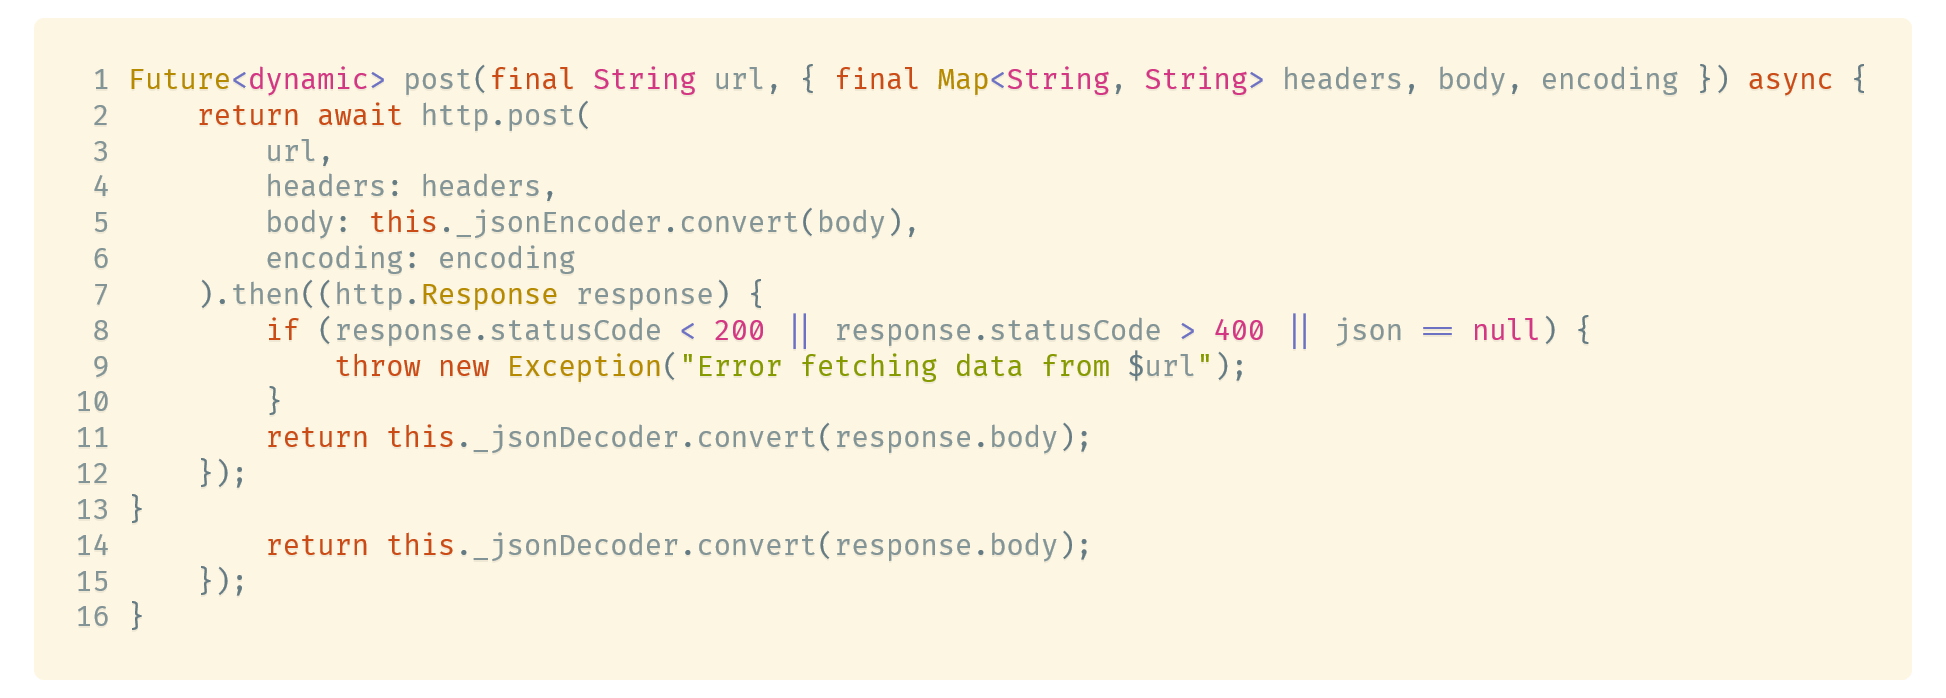
\includegraphics[width=1\textwidth]{images/Dart/util/network-wrapper/networkWrapperPOST.png}
    \caption{POST-Request-Wrapper der NetworkWrapper-Klasse}
\end{code}